\documentclass[10pt,twocolumn,letterpaper]{article}

\usepackage{cvpr}
\usepackage{times}
\usepackage{epsfig}
\usepackage{graphicx}
\usepackage{amsmath}
\usepackage{amssymb}

% Include other packages here, before hyperref.

% If you comment hyperref and then uncomment it, you should delete
% egpaper.aux before re-running latex.  (Or just hit 'q' on the first latex
% run, let it finish, and you should be clear).
\usepackage[pagebackref=true,breaklinks=true,letterpaper=true,colorlinks,bookmarks=false]{hyperref}

% \cvprfinalcopy % *** Uncomment this line for the final submission

\def\cvprPaperID{****} % *** Enter the CVPR Paper ID here
\def\httilde{\mbox{\tt\raisebox{-.5ex}{\symbol{126}}}}

% Pages are numbered in submission mode, and unnumbered in camera-ready
\ifcvprfinal\pagestyle{empty}\fi
\begin{document}

%%%%%%%%% TITLE
\title{Using fine-grain detection to understad society}

\author{First Author\\
Institution1\\
Institution1 address\\
{\tt\small firstauthor@i1.org}
% For a paper whose authors are all at the same institution,
% omit the following lines up until the closing ``}''.
% Additional authors and addresses can be added with ``\and'',
% just like the second author.
% To save space, use either the email address or home page, not both
\and
Second Author\\
Institution2\\
First line of institution2 address\\
{\tt\small secondauthor@i2.org}
}

\maketitle
%\thispagestyle{empty}

%%%%%%%%% ABSTRACT
\begin{abstract}
Detecting a large number of BMWs in images informs us that those images may be of a wealthy area. Conversely, knowing that our images were obtained from a wealthy neighborhood increases the likelihood of detecting expensive cars. We explore this relationship between demographic factors and fine-grain classes by performing large scale detection of over 2600 car classes and conducting a social analysis of unprecedented scale in computer vision. Using 45 million images from 200 of the biggest cities in the United States,we predict demographic factors such as neighborhood wealth and crime statistics. Finally we show that just as fine-grain classes provide demographic information, societal cues can assist in fine-grain classification and improve accuracy. To facilitate our work, we have collected the largest and most challenging fine-grain dataset reported to date consisting of 3147 classes of cars comprised of images from google streetview and other web sources and classified by car experts to account for even the most subtle of visual differences. We hope our work ushers in a new research area fusing fine-grained object detection and societal analysis.
\end{abstract}

\section{Introduction}
%%%%%%%%% BODY TEXT
The ubiquity of streetview images has jumpstarted a new line of computer vision research focused on understanding cities through images \cite{mit_plos_1}~\cite{MIT_vision}~\cite{tamara}. For example, \cite{mit_plos_1} that crime predictions can be improved by incorporating human perceptions of neighborhoods' images rather than using census data such as income alone~\cite{mit_plos_1} and ~\cite{tamara} and \cite{MIT_vision} learn these perceptions using computer vision techniques. However, in order to extend these methods to other cities,extensive annotations of millions of images from each city would be required since, as ~\cite{tamara} showed, algorithms trained on images of Boston, for example, cannot predict safety or wealth on images from San Francisco.  We explore the question of learning social priors using large scale fine-grain classifications of cars and show that many neighborhood statistics such as income and crime rate can be predicted from car detections. Furthermore, using our detections in conjunction with census data,we can answer questions like what types of cars do rich/poor people drive? 

\begin{figure}[t]
\begin{center}
\fbox{\rule{0pt}{2in} \rule{0.9\linewidth}{0pt}}
   %\includegraphics[width=0.8\linewidth]{egfigure.eps}
\end{center}
   \caption{Example of caption.  It is set in Roman so that mathematics
   (always set in Roman: $B \sin A = A \sin B$) may be included without an
   ugly clash.}
\label{fig:pull}
%\label{fig:onecol}
\end{figure}

Finally we show that we can use the answers to these questions to help improve fine-grained classification. Although an increasing number of images that we interact with daily are associated with GPS tags, there are very few computer vision algorithms that take advantage of location based metadata. This metadata can be especially important in fine grain classification. For example, just as detecting a large number of expensive cars in one area can give us a hint that we are in the vicinity of a wealthy neighborhood, knowing that we are in a wealthy neighborhood can also increase our likelyhood of detecting expensive cars. Similarly, knowing that we are in a farm area increases our liklihood of detecting farm related cars and seeing many family households with young children increases our likelihood of detecting SUVs. We show that this information can be leveraged to improve fine-grain classification. Although there has been previous work on learning spatio-temporal priors for fine-grain classification~\cite{birdsnap} and exploiting streetview geometry and GIS systems to improve object detection~\cite{nyc3D,amir} to our knowledge this is the first time census data and other social cues have been used to assist in fine-grain classification.  


Summarizing our contributions:
  \begin{enumerate}
    \item We perform a large scale analysis of cities using our car detections and present intuitive as well as interesting insights
    \item We show that using social cues extracted from census data can improve fine-grain classificaiton accuracy
    \item We present the largest fine-grain car dataset reported to our knowledge, complete with geotags and class as well as geography metadata  
    \item We include a larger set of 45 million streetview images with car detections and fine-grain class predictions
  \end{enumerate}

%-------------------------------------------------------------------------
%\begin{figure*}
%\begin{center}
%\fbox{\rule{0pt}{2in} \rule{.9\linewidth}{0pt}}
%\end{center}
%   \caption{Example of a short caption, which should be centered.}
%\label{fig:short}
%\end{figure*}

\begin{figure}[t]
\begin{center}
\fbox{\rule{0pt}{2in} \rule{0.9\linewidth}{0pt}}
   %\includegraphics[width=0.8\linewidth]{egfigure.eps}
\end{center}
   \caption{Example of caption.  It is set in Roman so that mathematics
   (always set in Roman: $B \sin A = A \sin B$) may be included without an
   ugly clash.}
\label{fig:data}
%\label{fig:onecol}
\end{figure}
%------------------------------------------------------------------------
\section{Related Work}
\textbf{Analysis of cities using images.}
  \begin{enumerate}
     \item Plos one journal from MIT asking people to predict whether an area is safe/wealthy etc... after looking at the images
     \item streetscore MIT paper predicting safety wealth scores etc.. just from images~\cite{MIT_vision}
     \item tamara Berg's paper on safety on ECCV
     ~\cite{zhang2014part}
     ~\cite{caltech_birds}
\textbf{Using GPS data to improve object detection.}
     \item Amir's work in GIS assisted object detections. For objects like streetlamps and trashcans, uses GIS to reproject objects to a plane and reduce the search space for object detection .
     \item NYC 3D uses geographic elevation data to create view-point aware detectors and extract ground planes for  them

  \end{enumerate}

%------------------------------------------------------------------------
\section{Cars and Cities dataset}
Our dataset consists of W number of images annotated with bounding boxes and fine-grained classes for training and validating fine-grained car detectors and 45 million streetview images for societal analysis.

\subsection{Images with Labeled fine-grained classes}
Out of the images annotated with fine-grained classes and bounding boxes, X were obtained from google streetview, Y from craigslist.com and Z from cars.com. A of our images have bounding boxes for cars and B are annotated with fine-grain labels. The bounding boxes were obtained through a series of AMT tasks. The fine-grain labels were created by first coming up with a classlist of 18000 cars comprising of all cars listed on edmunds.com and grouping them into visualy indistinguishable sets of groups using a series of amazon mechanical turk tasks as well as manual labor by the authors. After creating an exhaustive class list of 3147 classes, images from craigslist and cars.com were labeled by parsing the posting titles while cars from google streetview were labeled using 100 hired car experts.

\begin{figure}[t]
\begin{center}
\fbox{\rule{0pt}{2in} \rule{0.9\linewidth}{0pt}}
   %\includegraphics[width=0.8\linewidth]{egfigure.eps}
\end{center}
   \caption{Example of caption.  It is set in Roman so that mathematics
   (always set in Roman: $B \sin A = A \sin B$) may be included without an
   ugly clash.}
\label{fig:dataset1}
%\label{fig:onecol}
\end{figure}

\begin{figure}[t]
\begin{center}
\fbox{\rule{0pt}{2in} \rule{0.9\linewidth}{0pt}}
   %\includegraphics[width=0.8\linewidth]{egfigure.eps}
\end{center}
   \caption{Example of caption.  It is set in Roman so that mathematics
   (always set in Roman: $B \sin A = A \sin B$) may be included without an
   ugly clash.}
\label{fig:dataset2}
%\label{fig:onecol}
\end{figure}

\begin{figure}[t]
\begin{center}
\fbox{\rule{0pt}{2in} \rule{0.9\linewidth}{0pt}}
   %\includegraphics[width=0.8\linewidth]{egfigure.eps}
\end{center}
   \caption{Example of caption.  It is set in Roman so that mathematics
   (always set in Roman: $B \sin A = A \sin B$) may be included without an
   ugly clash.}
\label{fig:dataset3}
%\label{fig:onecol}
\end{figure}

Fig.~\ref{fig:dataset1} shows example images from our data while Fig.~\ref{fig:dataset2} shows some image statistics. Images from craigslist.com and cars.com have one large bounding box whereas google streetview images have multiple small boxes with cars that are blurred and occluded. As shown in Fig.~\ref{fig:dataset3} the different finegrained classes are very difficult to distinguish

\subsection{Images with no labeled fine-grained classes}
In order to perform societal analysis, we collected 45 million google streetview images from 8 million points in 200 of the biggest cities in the United States. These images were collected by sampling latitude,longitude points on roads, spaced 25 meters apart. Fig.~\ref{fig:dataset4} shows maps from two cities with the samples that were collected and fig.~\ref{fig:dataset5} shows the number of samples for the 10 biggest cities. For each sample, we collect images at 0,60,120,180,240,300 degrees.

\begin{figure}[t]
\begin{center}
\fbox{\rule{0pt}{2in} \rule{0.9\linewidth}{0pt}}
   %\includegraphics[width=0.8\linewidth]{egfigure.eps}
\end{center}
   \caption{Example of caption.  It is set in Roman so that mathematics
   (always set in Roman: $B \sin A = A \sin B$) may be included without an
   ugly clash.}
\label{fig:dataset4}
%\label{fig:onecol}
\end{figure}

\begin{figure}[t]
\begin{center}
\fbox{\rule{0pt}{2in} \rule{0.9\linewidth}{0pt}}
   %\includegraphics[width=0.8\linewidth]{egfigure.eps}
\end{center}
   \caption{Example of caption.  It is set in Roman so that mathematics
   (always set in Roman: $B \sin A = A \sin B$) may be included without an
   ugly clash.}
\label{fig:dataset5}
%\label{fig:onecol}
\end{figure}

\section{Car detection and fine-grained classification}
In order to detect and classify 45 million images, we need to use an efficient car detection and classification algorithm. Although RCNN ~\cite{rcnn} has been shown to be state of the art in object detection, it's memory and computation requirement make it impossible for use in a large scale detection problem such as ours. Specifically training with RCNN  would require XXXXGB of memory and XXXX GPUs and car detection on 45 million images would take XXminutes per bounding box on XXX machine. We therefore used a simple DPM model with 0 components to detect cars and a standard CNN from Alex etal ~\cite{alexnet} to perform classification on the detected bounding boxes. As shown in Fig.~\ref{fig:dpm_acc} there is only an XX\% drop in average precision between using a dpm with 0 components and 0 parts and one with XXX components and YYY parts.

\begin{figure}[t]
\begin{center}
\fbox{\rule{0pt}{2in} \rule{0.9\linewidth}{0pt}}
   %\includegraphics[width=0.8\linewidth]{egfigure.eps}
\end{center}
   \caption{Example of caption.  It is set in Roman so that mathematics
   (always set in Roman: $B \sin A = A \sin B$) may be included without an
   ugly clash.}
\label{fig:dataset5}
%\label{fig:onecol}
\end{figure}

In order to classify the detected cars, we train a standard CNN from ~\cite{alexnet} using caffe ~\cite{caffe}.Although our aim is to train fine-grain detections for streetview images, many of our training images are obtained from other web sources due to the fact that annotating streetview images is expensive. Thus we apply various deformations such as blurring and aspect ratio distortion in an attempt to deform the web images into streetview images. Table~\ref{table:acc-deformation} shows the obtained accruacy after adding each deformation. During test time, we classify the top 10\% scoring dpm bounding boxes using our CNN. This speeds up classification time by 10X while only resulting in a drop of .5 AP. 

\begin{table}
\begin{center}
\begin{tabular}{|l|c|}
\hline
Method & Frobnability \\
\hline\hline
Theirs & Frumpy \\
Yours & Frobbly \\
Ours & Makes one's heart Frob\\
\hline
\end{tabular}
\end{center}
\caption{Results.Ours is better.}
\label{table:acc-deformation}
\end{table}

\section{Societal analysis}
\label{sec:social}
After collecting data, training fine-grained car detectors and classifying cars in all of our images, we are now ready to perform some social analysis. We show some general results from the entire united states as well as a case study from Massachussettes.

We gathered zipcode level as well as census tract level 2007-2012 American Community Survey data for the 200 cities in our dataset and analyzed how the census data relates to statistics from our detected cars. As shown in fig.~\ref{fig:corrs}, median household income is highly correlated with the average price of cars in a given zip code (Pearson correlation 0.493, P-value of T-Test \(<< 0.001\). The correlation coefficient varies city by city from 0.8 for city XXXX to 0.4 for city YYY. 

\begin{figure}[t]
\begin{center}
%\fbox{\rule{0pt}{2in} \rule{0.9\linewidth}{0pt}}
   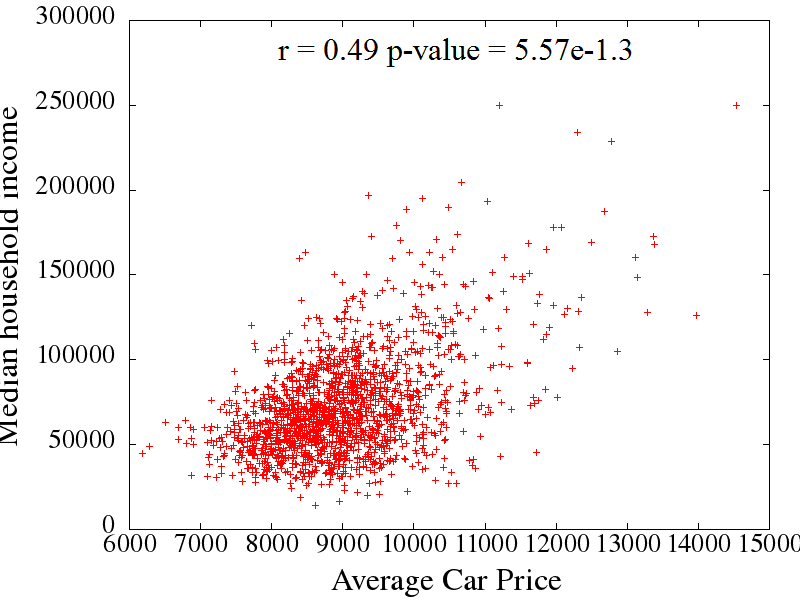
\includegraphics[width=0.8\linewidth]{img/averagePriceIncome.png}
\end{center}
   \caption {Average car price w.r.t. median household income.}
\label{fig:corrs}
%\label{fig:onecol}
\end{figure}

\subsection{What do poor people drive and what do rich people drive?}
We found a strong positive correlation (Pearson Correlation 0.592, P-value of T-Test \(<< 0.001\) between the percentage of cars made outside of the United States and the median household income per zip code. As shown in Figure \ref{fig:cartoincome} (A), rich people seem to drive German cars (Pearson correlation 0.57) where as there is a surprising strong negative correlation of -0.59 between the number of American cars per zip code and median household income even though the number of American cars in our dataset is higher than the number of German cars. 

Not surprisingly, rich people also dirve newer cars. Figure \ref{fig:cartoincome} B shows the correlations between the number of cars in different year bins vs. median household income. Starting with a strong negative correlation of -0.4 between the number of cars from 1990-1994 in a given zipcode and median household income, the correlation keeps on increasing for newer cars reaching a small positive value for cars in 2000-2004 and a maximum value of 0.46 for cars in 2000-2013. 
 

\begin{figure}[t]
\begin{center}
%\fbox{\rule{0pt}{2in} \rule{0.9\linewidth}{0pt}}
    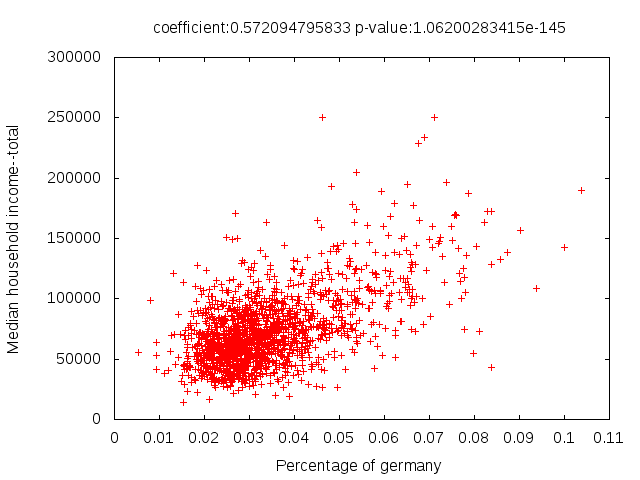
\includegraphics[width=0.3\linewidth]{img/germanyIncome.png}
    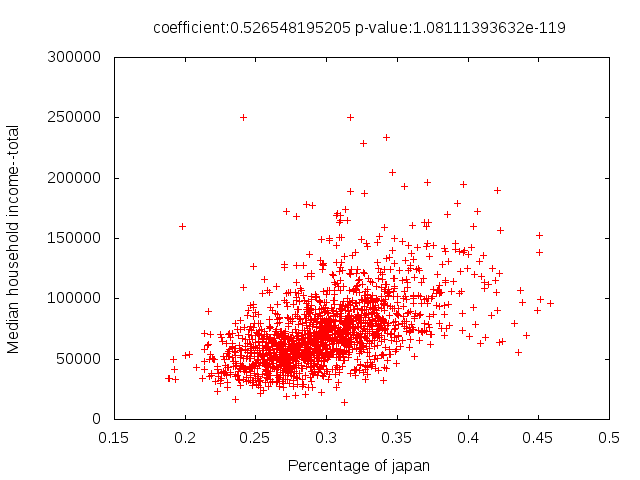
\includegraphics[width=0.3\linewidth]{img/japanIncome.png}
    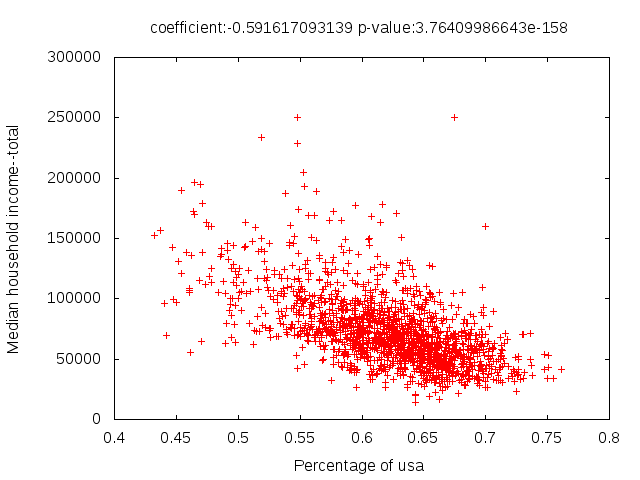
\includegraphics[width=0.3\linewidth]{img/usaIncome.png}
    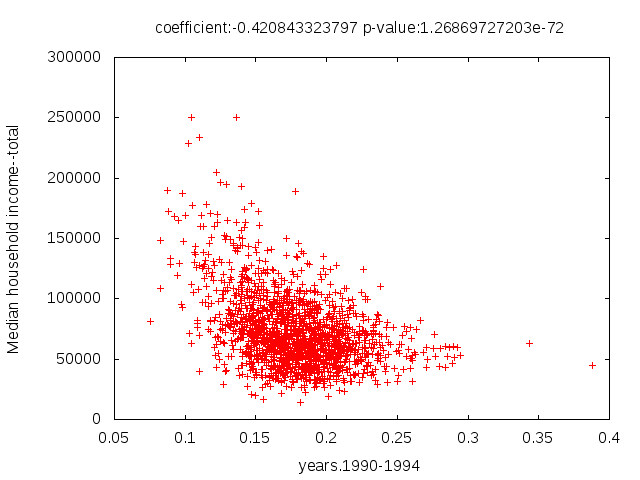
\includegraphics[width=0.3\linewidth]{img/years1990-1994Income.png}
    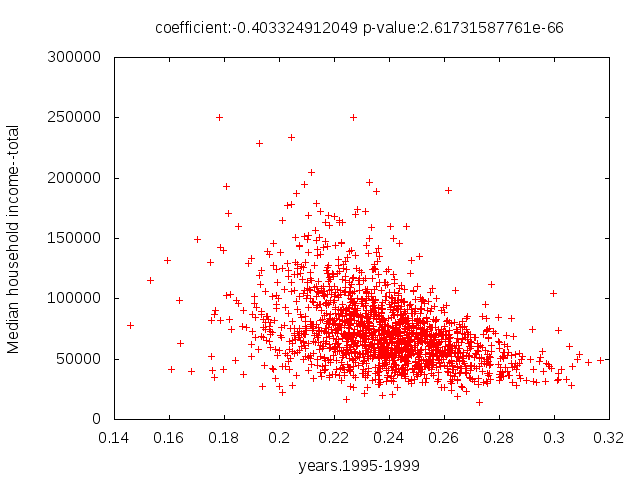
\includegraphics[width=0.3\linewidth]{img/years1995-1999Income.png}
    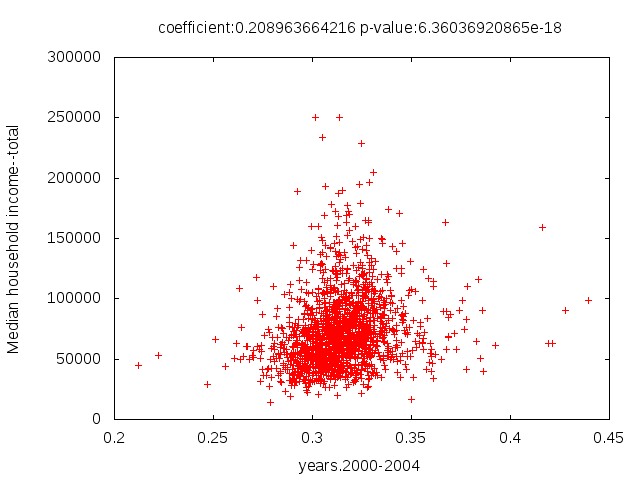
\includegraphics[width=0.3\linewidth]{img/years2000-2004Income.png}
    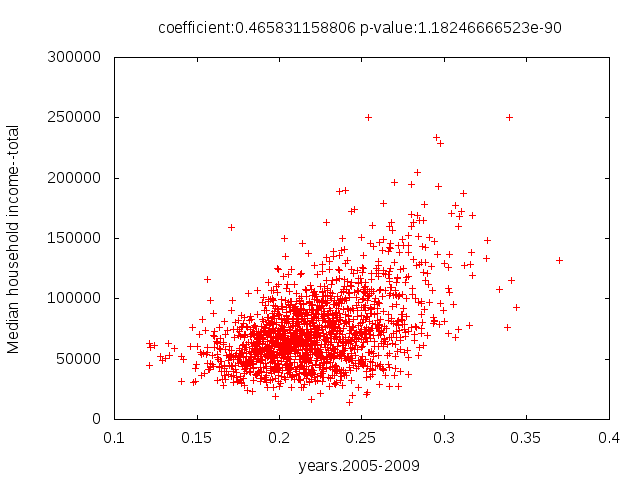
\includegraphics[width=0.3\linewidth]{img/years2005-2009Income.png}  
    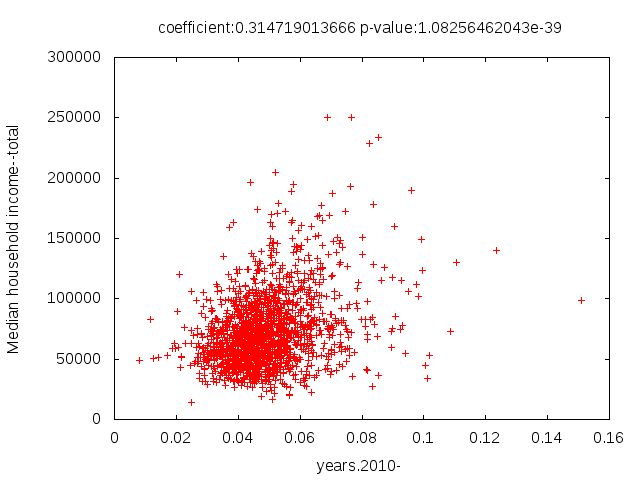
\includegraphics[width=0.3\linewidth]{img/years2009-2013Income.png}  
    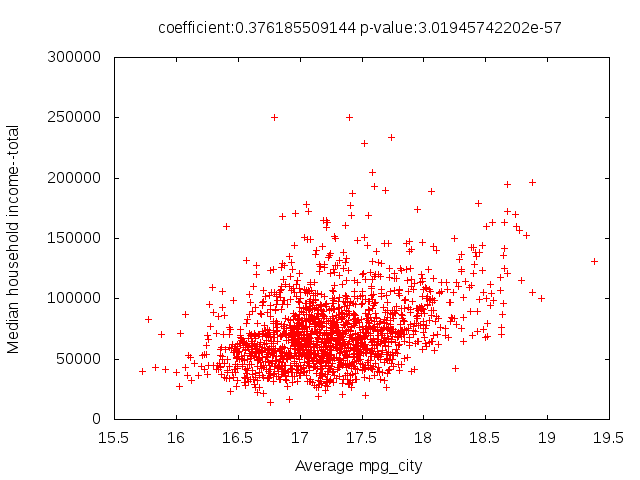
\includegraphics[width=0.3\linewidth]{img/mpg_cityIncome.png}  
\end{center}
   \caption {(A) Countries of cars vs. median household income, (B) years of cars vs. median household income, (C) years of cars vs. median household income, last column is avg. city MPG vs. median household income}
\label{fig:cartoincome}
%\label{fig:onecol}
\end{figure}

Finally, as shown in figure ~\ref{fig:cartoincome} C poor people live in zipcodes with cars that have low mileage while rich people live in zipcodes having cars with high MPG. As shown in ~\cite{pollution_race_ca} poor people are exposed to higher levels of pollution because they live near areas with higher traffic levels and cars with high C02 emissions. Finally Figure \ref{fig:pricetoedu}, shows the relationship between education and the average car price of detected cars in a zipcode. There is a moderate negative correlation of -0.211 between highschool educated people and the price of the car in their zipcode as opposed to a positive correlation of 0.319 between the number of graduate school educated people in a zipcode vs. the average car price. As expected, the jump in correlation coefficient from high school educated to college educated (-0.21 to 0.32) is higher than the jump from college educated to graduate school educated (0.32-0.39). Although we have found many interesting results, we will cover them in the supplemental material for the sake of brevety.


\begin{figure}[t]
\begin{center}
%\fbox{\rule{0pt}{2in} \rule{0.9\linewidth}{0pt}}
    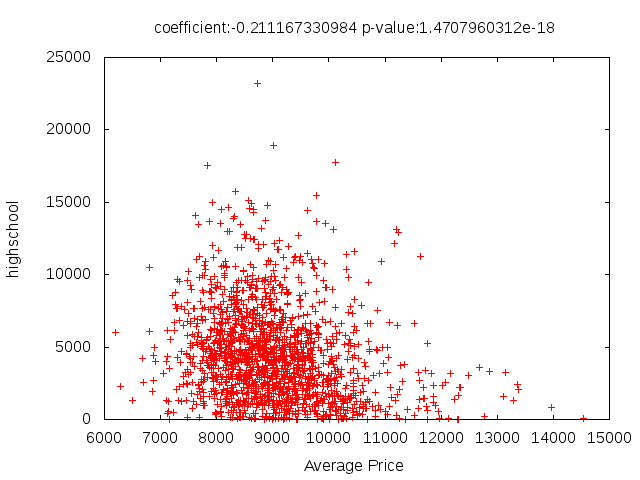
\includegraphics[width=0.3\linewidth]{img/averagePriceHighSchool.png}
    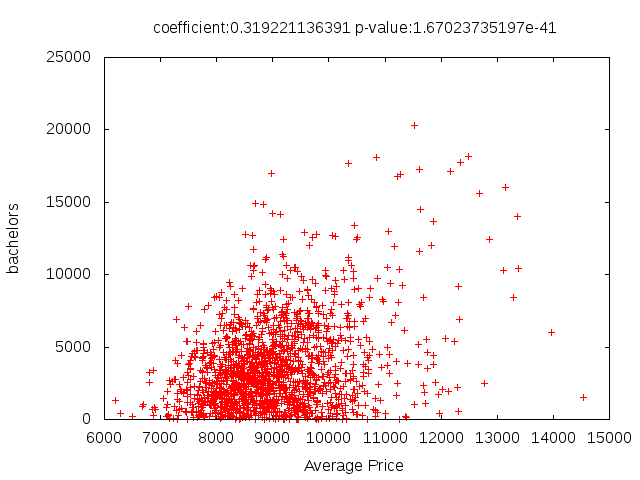
\includegraphics[width=0.3\linewidth]{img/averagePriceBachelor.png}
    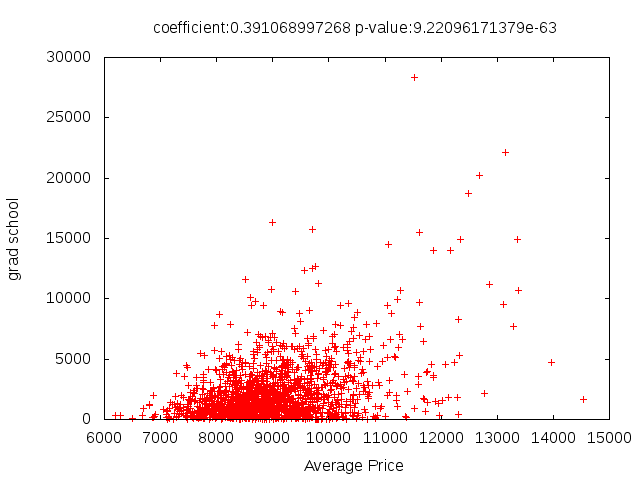
\includegraphics[width=0.3\linewidth]{img/averagePriceGradSchool.png} 
\end{center}
   \caption {Number of people with different education level vs. average car price per zipcode}
\label{fig:pricetoedu}
%\label{fig:onecol}
\end{figure}

\subsection{Which neighborhoods are wealthy/poor?}
We found that the results of our fine-grained car detections can be used to learn various attributes of neighborhoods. Intuitively, if we see many expensive cars on the street, we suspect that we are in a rich neighborhood and viceversa. However, the correlation between car prices and neighborhood wealth is not going to be perfect because we are not necessarily detecting the cars that residents drive. Figure \ref{fig:bosvis} shows a heatmap of the average price of detected cars within a zipcode and median household income in a zipcode. We can see that just by looking at the average price of cars within a zipcode we can correctly predict most of the high and low income zipcodes. We show these viusalizations for all 200 cities in our supplemental material and only present two cities here.


\subsection{Which cities are more segregated?}
Following the analysis of~\cite{mit_plos_1} we use Getis Gi* statistic to produce statistically significant clusters of expensive and cheap cars and use Moran's I statistic ~\cite{moran} to measure the spatial seggregation of car price with values ranging from -1 to 1. A value of -1 indicates perfect anti-correlation like a checkerboard where as a value of 1 indicates that similar values are perfectly clustered. The null hypothesis of complete spatial randomness produces values near 0. After creating a z-score for Moran's statistic we see that Boston, for example has a higher z-score than **XXX** showing that Boston has more seggreaged neighborhoods than **XXX**. After measuring the length of the spatial autocorrelation function of the average car price per zipcode and calculating the correlation length, we find that *XXXX* is found to be the city with the highest correlation length, and therefore the city with the most seggregated neighborhoods by income which is corroborated by census data ~\cite{census-segreggation}. Fig. ~\ref{fig:boston-hotspot}A shows statistically significant clusters of high and low car prices in Boston and Fig.~\ref{fig:autocorr} shows spatial correlograms for 5 cities displaying the decay of spatial autocorrelation as a function of distance.

\begin{figure}[t]
\begin{center}
%\fbox{\rule{0pt}{2in} \rule{0.9\linewidth}{0pt}}
    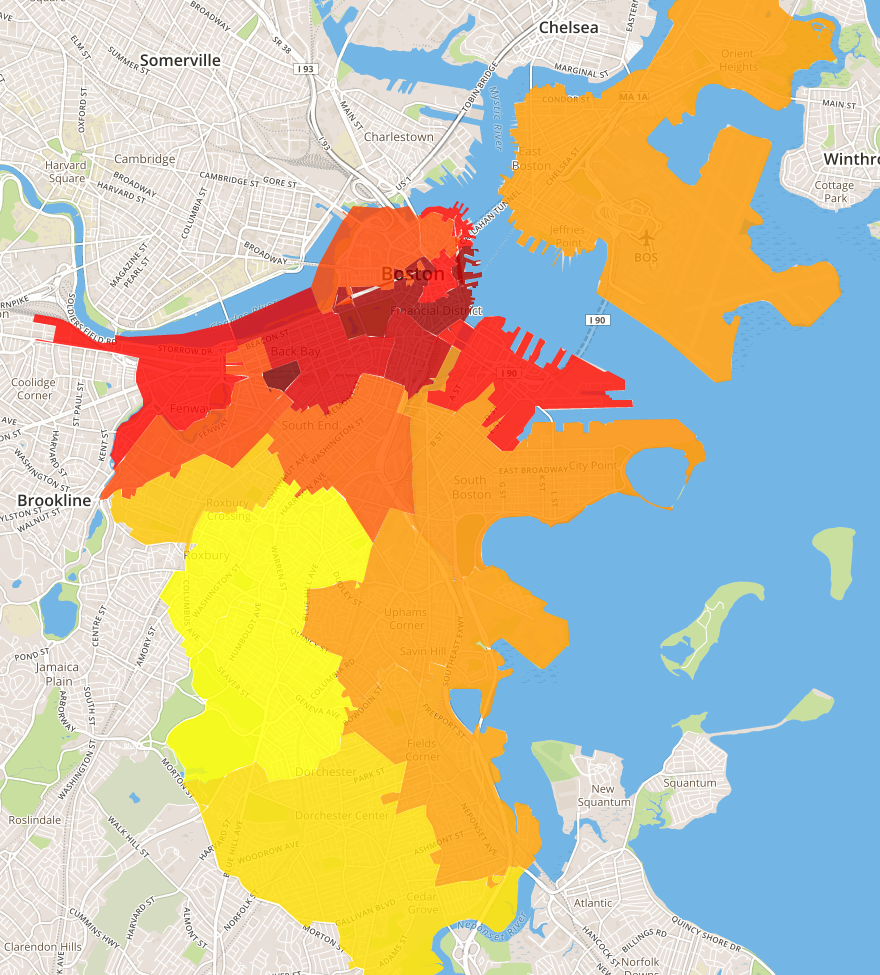
\includegraphics[width=0.45\linewidth]{img/price.png}
    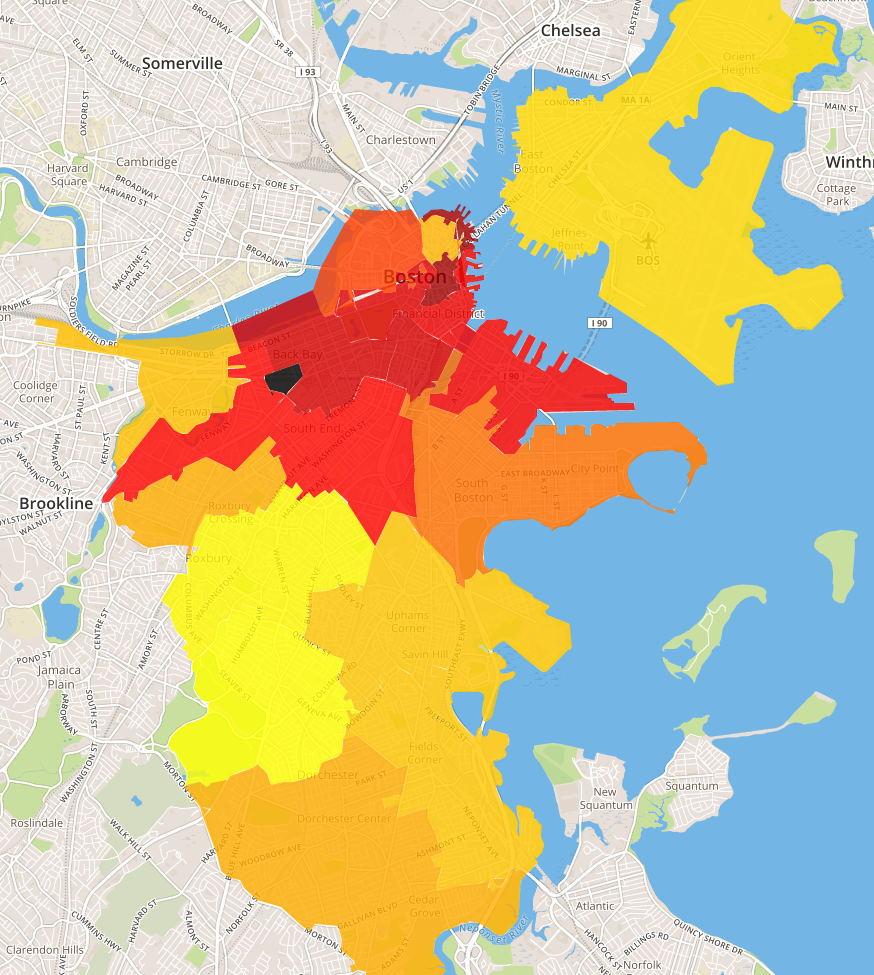
\includegraphics[width=0.45\linewidth]{img/income.png}
\end{center}
   \caption {(A) Heatmap of average car price in Boston. (B) Heatmap of median household income in Boston}
\label{fig:bosvis}
%\label{fig:onecol}
\end{figure}

\begin{figure}[t]
\begin{center}
%\fbox{\rule{0pt}{2in} \rule{0.9\linewidth}{0pt}}
    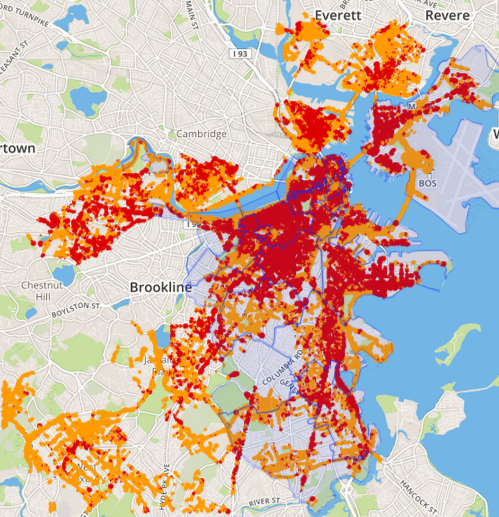
\includegraphics[width=0.45\linewidth]{img/boston-hotspot.png}
    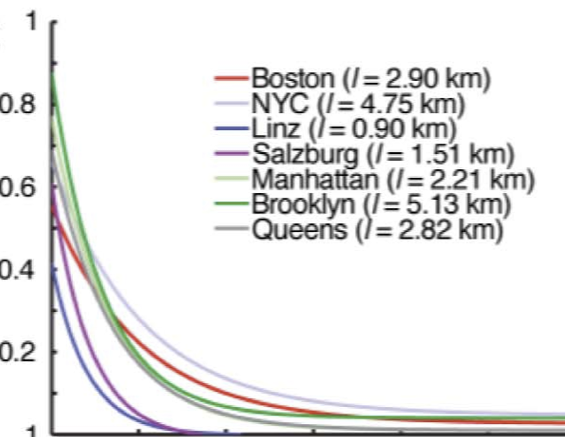
\includegraphics[width=0.45\linewidth]{img/autocorr.png}
\end{center}
   \caption {(A)  Map of Boston showing statistically significant clusters of high -and low- car parices according to Getis Gi* statistic. Red shows clusters of high prices and orange shows clusters of low prices. (B) Spatial correlograms showing the decay of spatial autocorrelation as a function of distance.}
\label{fig:boston-hotspot}
%\label{fig:onecol}
\end{figure}

\section{Using social priors to improve classification}
As shown in section ~\ref{sec:social} there is a very high correlation between some census variables such as income, and car attributes such as price and year. Given this relationship, we explore the use of census data to improve our fine-grain classification.

\subsection{Analyzing classification accuracy}
Since census data is most highly correlated with aggregate car attributes, one question is how much knowing ground truth car attributes would help in classification accuracy. This gives us an upper bound for the gain in accuracy that can be obtained by using census variables as a prior. Table~\ref{table:car-att} lists the classification accuracy after using ground truth car attributes. Surprisingly, knowing the manufacturing country of the car gives very little gain in accuracy (\(\sim\) 0.5\%). However, localizing the car price to within one of two bins of expensive vs cheap cars provides a gain in accuracy of ~3\%. Looking at the confusion matrices in fig. ~\ref{fig:fg-confusion} we can see that after dividing the car price into 5 bins using quantiles, some expensive cars are confused with cheap cars where as most car countries of origin are not confused with other countries, except for one case of confusion between South Korean and Japanese cars.

\begin{figure*}[t]
\begin{center}
   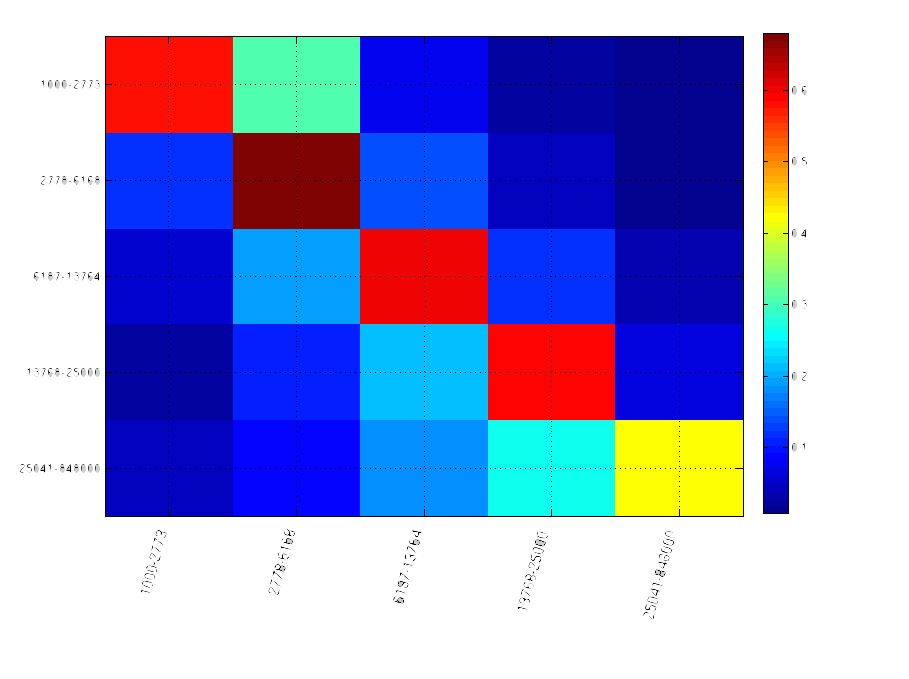
\includegraphics[width=0.4\linewidth]{img/confusion_price5.png}
   \hspace{0.1\linewidth}
   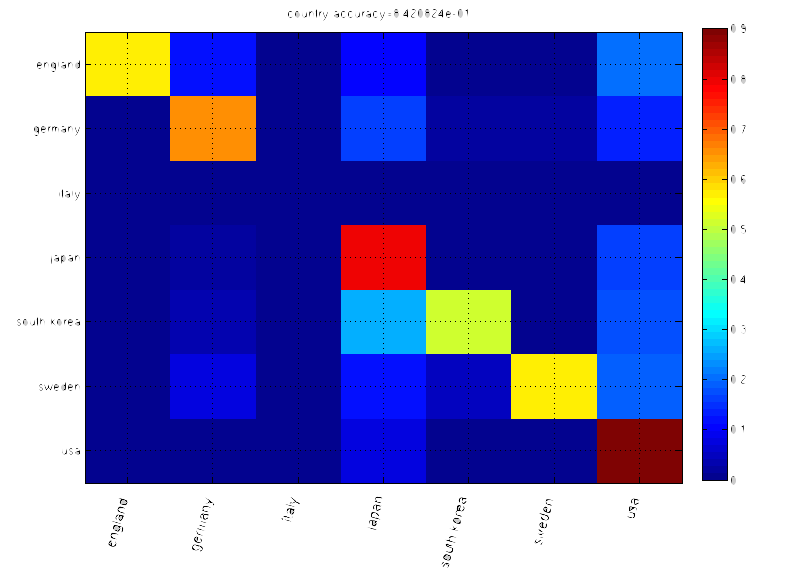
\includegraphics[width=0.4\linewidth]{img/confusion_country.png}
\end{center}
   \caption{(A) Confusion matrix between different price bins. Cheap cars are mistaken for expensive cars (B) Between cars made in different countries}
\label{fig:fg-confusion}
\end{figure*}

We take this experiment further and plot accuracy Vs. price bin in fig.~\ref{fig:price-acc} for various numbers of price bins, all generated using quantiles, localized to various degrees of accuracy. For example, we can see that if we localize
 the price of the car to one of 4 bins we would get an 8\% increase in classification accuracy. However, even localizing 
the price to within 3 out of those 4 bins would result in a ~1\% increase.


\begin{table}
\begin{center}
\begin{tabular}{|l|c|}
\hline
Method & Frobnability \\
\hline\hline
Theirs & Frumpy \\
Yours & Frobbly \\
Ours & Makes one's heart Frob\\
\hline
\end{tabular}
\end{center}
\caption{Classification accuracy with ground truth attributes}
\label{table:car-att}
\end{table}

\begin{figure}[t]
\begin{center}
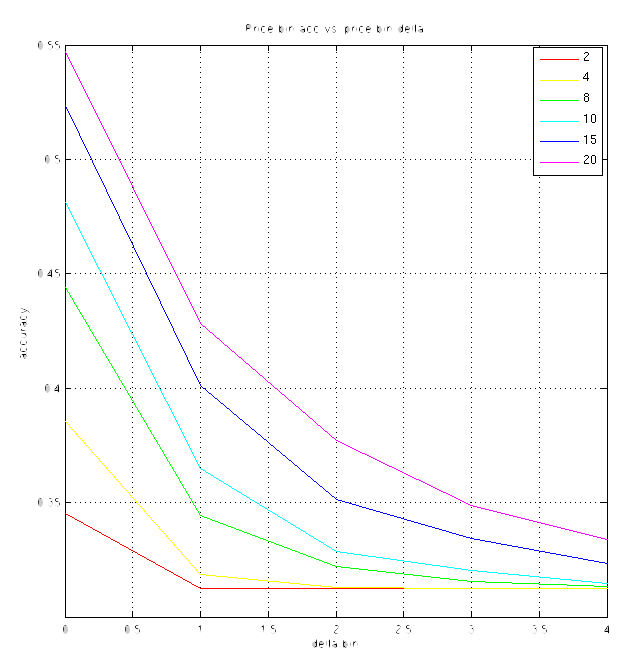
\includegraphics[width=0.9\linewidth]{img/price-att.png}
\end{center}
   \caption{Fine-grain classification accuracy with ground truth price bin. X axis is the number of bins to which the price is localized and Y axis is classification accuracy. For example, localizing the price to 3 out of 8 bins results in a classification accuracy of 33\% which is 2\% higher than the baseline, 31.27\%}
\label{fig:price-acc}
\end{figure}

\subsection{Using census priors to predict attributes}
\label{sec:prior-att}
As shown in ~\cite{birdsnap} ~\cite{Other context stuff} using contextual priors can improve object classification accuracy. In order to directly use census information as a prior, we would like to find \(P(C|I,Sk)\) where \(C\) is the fine-grain class,\(I\) is an image and \(Sk\) \(\in\) \(\{\)\(S1\) \ldots \(Sn\)\(\}\) is a particular zip code level census variable such as median household income. Using Bayes' rule:
\begin{equation}
P(C|I,Sk)=\frac{P(I,Sk|C)P(C)}{P(I,Sk)}
\end{equation}
If we assume that the image and census data are conditionally independent given the fine-grained class label, the above equation can be written as 
\begin{equation}
P(C|I,Sk)=\frac{P(I|C)P(Sk|C)P(C)}{P(I,Sk)}
\end{equation}
After applying Bayes' rule again to \(P(I|C)\) and \(P(Sk|C)\) , we get 
\begin{equation}
P(C|I,Sk)=\frac{P(C|I)P(I)}{P(C)}\frac{P(C|Sk)P(Sk)}{P(C)} \frac{P(C)}{P(I,Sk)}
\end{equation}
\begin{equation}
\propto \frac{P(C|I)}{P(C)}P(C|Sk)
\label{eq:prior-eq}
\end{equation}

We experimented with different methods of using census variables as priors. The first method was to quantize them into varying numbers of bins and calculate \(P(C|Sk)\) in equation ~\ref{eq:prior-eq} for each census variable.As shown in table ~\ref{table:prior-acc} this method results in a reduction in accuracy because we do not have enough geotagged training data to gain informative knowledge from the census about one of 2657 fine-grain classes. However, although there are 2657 classes, the number of attribute classes is much lower. If \(Aj\) \(\in\) \(\{\) \(A1\) \ldots \(An\)\(\}\) represents a car attribute such as price, we can reformulate \(P(C|Sk)\) in equation~\ref{eq:prior-eq} as \(P(C|Aj)\)\(P(Aj|Sk)\). This formulation comes from a naive bays generative model assuming that \(Sk\) are the observed variables from which we can calculate \(P(Aj|Sk)\). After this modification, equation ~\ref{eq:prior-eq} can be written as


\begin{equation}
  P(C|I,Sk) \propto \frac{P(C|I)}{P(C)}P(C|Aj)P(Aj|Sk)
\end{equation}
We calculate \(P(C|I,Sk)\) for all car attributes and 30 different census variables, quantizing them into bins ranging from 2-20. Table~\ref{table:prior-acc} shows the 3 highest accuracy numbers for various combinations of census variables and car attributes. It can be seen that using median household income and either car price or year result in the highest accuracy gain (although this gain is very slight). This result is to be expected given the social analysis results of section~\ref{sec:social} showing high correlation between median household income and car price and year.


\subsection{Multiple car attributes and census variables}
In section \ref{sec:prior-att} we used single car attributes and census variables to calculate prior probabilities. We also experimented with using multiple census variables to predict single car attributes as well as combining priors independently calculated from multiple census variables and car attributes. To obtain \(P(Aj|S1...Sn)\) we first quantize attributes \(Aj\) into \(M\) bins where \(M\) ranges from 2 to 20. If \(Aj\) has a fixed number of classes (such as car make), \(M\) is just the number of attribute classes. We then perform multi-class logistic regression along with feature selection to classify \(Aj\) into one of \(M\) bins using \(S1\) \ldots \(Sn\). \(P(Aj|S1\) \ldots \(Sn)\) is then the probability obtained through logistic regression.

Finally, we combine the priors learned for different attributes by using the fact that car attributes are independent from each other given the class. Using this assumption along with Bayes’ rule \(P(C|A1 \ldots An)\) can be written as 

\begin{equation}
\frac{P(A1\ldots An|C)P(C)}{P(A1\ldots An)}
\end{equation}
After making use of the conditional independence of \(A1\) \ldots \(An\) given \(C\) this becomes
\begin{equation}
\frac{P(C)}{P(A1\ldots An)}\prod\limits_{j=1}^n P(Aj|C)
\end{equation}
And after applying Bayes’ rule to \(P(Aj|C)\) we get 
\begin{equation}
\propto \frac{P(C)}{P(A1\ldots An)}\prod\limits_{j=1}^n P(C|Aj)
\end{equation}

We assume that car attributes are independent from each other given census variables. \(P(C|I,S1 \ldots Sn)\) is then  

\begin{equation}
\propto \frac{P(C)}{P(A1\ldots An)}\prod\limits_{j=1}^n P(C|Aj)P(Aj|S1...Sn)
\end{equation}

Where \(P(Aj|S1...Sn)\) is given by the logistic regression probabilities.

Table XXX shows the accuracies obtained after combining multiple census attributes and multiple car attributes. ***Maybe more descussion after experiments***
\begin{table}
\begin{center}
\begin{tabular}{|l|c|}
\hline
Method & Frobnability \\
\hline\hline
Theirs & Frumpy \\
Yours & Frobbly \\
Ours & Makes one's heart Frob\\
\hline
\end{tabular}
\end{center}
\caption{Results.Ours is better.}
\label{table:prior-acc}
\end{table}

\section{Conclusion}
{\small
\bibliographystyle{ieee}
\bibliography{egbib}
}

\end{document}

{\small
\bibliographystyle{ieee}
\bibliography{egbib}
}
\end{document}

